\section{RESULTS}
This section compares comfort performance and time-varying occupancy density (Figures~\ref{fig:comfort} and~\ref{fig:OccuDensity}), then examines the magnitude and frequency of real-time setpoint changes (Figures~\ref{fig:control} and~\ref{fig:turnover_action}).

\subsection{Comfort performance across aggregation resolutions}
\begin{figure}[!htbp]
  \centering
  
\includegraphics[width=0.98\linewidth]{fig1_analysis23nr_with_fixed24_raw2000_64_100_all_solid_small_markers_paper}
  % {fig1_comfort_probability_64_100_paper}
  \caption{Mean person-time comfort probability under the three GCM policies and fixed baseline.}
  \label{fig:comfort}
\end{figure}
\begin{figure}[!htbp]
  \centering
  
\includegraphics[width=0.98\linewidth]{occupancy_density_timeofday_k12_paper}
  \caption{Decision-time occupancy density $N_{r,t}/K$ by time of day; lines show means, with 95\% confidence and simulation intervals}
  \label{fig:OccuDensity}
\end{figure}
Figure~\ref{fig:comfort} shows the same policy ranking in all four analyzed rooms: RT-GCM led at every $K$, followed by DGCM, while SGCM tracked near the fixed 24$^\circ$C baseline, steady at 65--70\% regardless of $K$.
RT-GCM declined from 96--97\% at $K=2$ to 79--82\% at the largest tested $K$; DGCM declined from 91--94\% to 72--76\%; SGCM fell from 72--73\% to 64--66\%, converging on the baseline.
Figure~\ref{fig:OccuDensity} shows that mean decision-time occupancy density remained below full occupancy and varied by room and time.
Thus, large member pools often produced partial attendance, allowing the present group to differ from regular membership and daily attendees and preserving an advantage for attendance-aware aggregation.

\subsection{Setpoint adjustments and occupant turnover}

Figure~\ref{fig:control}(a) relates daily mean occupancy to the magnitude of RT-GCM setpoint changes when a change occurred.
The central trend decreased from about 1.3$^\circ$C near a daily mean occupancy of one to roughly 1.0$^\circ$C near four and 0.8$^\circ$C at the highest observed daily mean occupancy, with the widest bands at low occupancy.
The typical step remained above the common 0.5$^\circ$C thermostat resolution.
Figure~\ref{fig:control}(b) resolves the same changed-step magnitude by $K$ and normalized daily mean occupancy $\bar N_d/K$.
The larger steps were concentrated at low normalized occupancy and generally declined as occupancy increased across $K$, consistent with Figure~\ref{fig:control}(a).

\begin{figure}[!htbp]
  \centering
  \begin{minipage}[t]{0.49\linewidth}
    \centering
    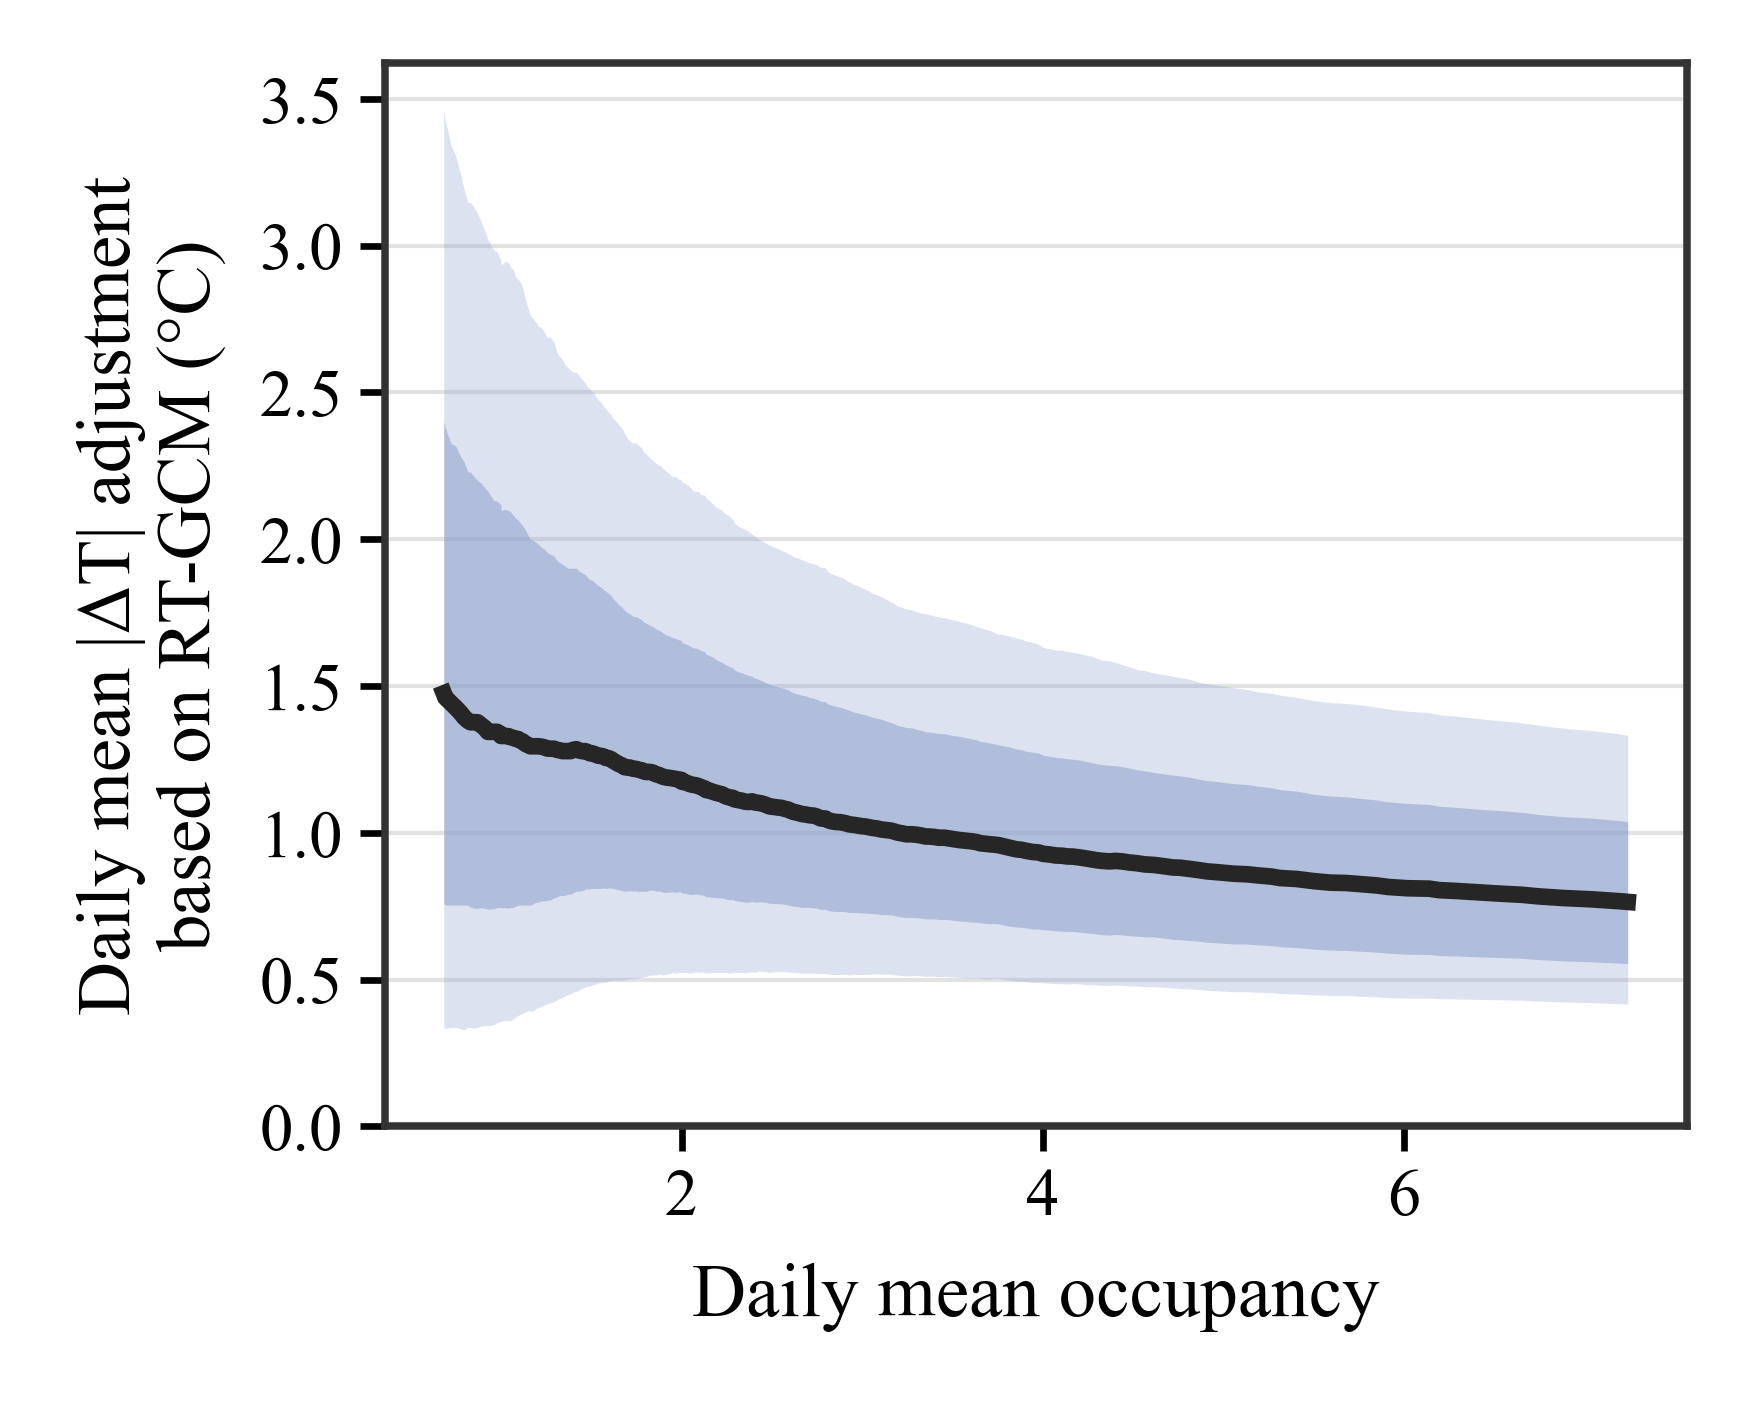
\includegraphics[width=\linewidth]{figures/fig3a_setpoint_adjustment_by_occupancy_compact_paper.png}
    \parbox{0.98\linewidth}{\centering (a) Mean absolute setpoint adjustment versus daily mean occupancy}
  \end{minipage}\hfill
  \begin{minipage}[t]{0.49\linewidth}
    \centering
    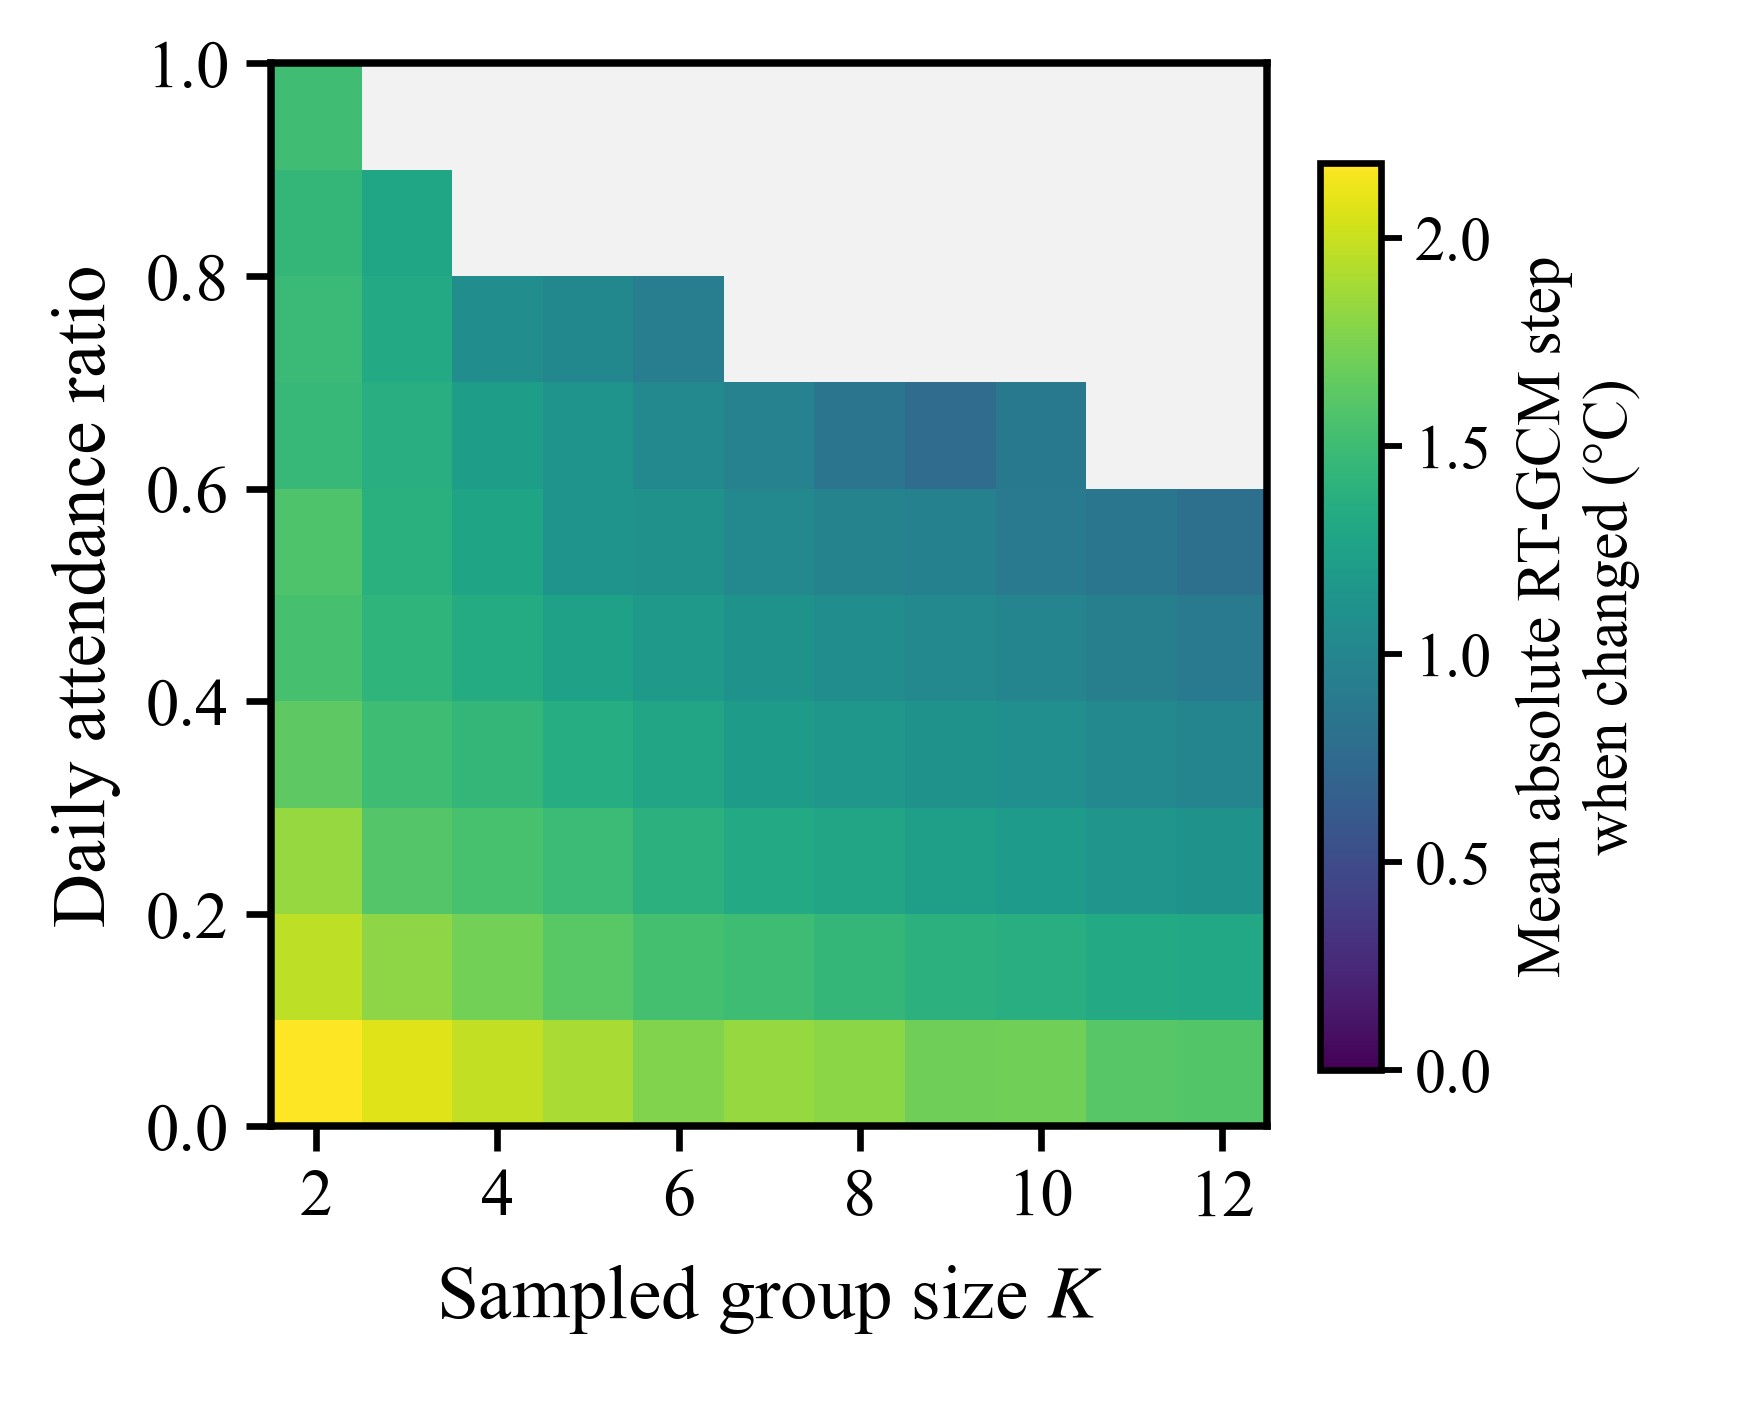
\includegraphics[width=\linewidth]{figures/fig3b_setpoint_adjustment_by_group_size_and_occupancy_density_compact_paper.png}
    \parbox{0.98\linewidth}{\centering (b) Mean absolute setpoint adjustment across $K$ and normalized daily mean occupancy, $\bar{N}_d/K$}
  \end{minipage}
    \caption{RT-GCM setpoint-change magnitude across occupancy conditions. (a) Daily mean absolute  setpoint change, versus daily mean occupancy; bands denote the 25--75\% and 10--90\% percentile ranges. (b) The same metric across $K$ and normalized daily mean occupancy $\bar N_d/K$; blank cells indicate insufficient observations.}
  \label{fig:control}
\end{figure}

Figure~\ref{fig:turnover_action}(a) relates occupant turnover to the frequency of actionable RT-GCM updates (at least 0.5$^\circ$C).
The horizontal axis is the 15-minute UTR, where zero indicates no change in occupant composition and one indicates complete replacement.
The vertical axis is the percentage of consecutive control intervals in which the RT-GCM setpoint changed by at least 0.5$^\circ$C.
The actionable-step rate increased monotonically from about 37\% at UTR near 0.05 to 63--69\% at 0.4, 77--78\% at 0.65, and 89--93\% at 0.9--1.0.
The near-overlap of the $K$ bands indicates that occupant replacement, rather than group size, was the dominant driver of short-interval action frequency.
Shared offices turned over dynamically through office hours, while the assigned-seat office (5A) stayed near 0.2--0.4 UTR and rarely reached the highest bins.
Figure~\ref{fig:turnover_action}(b) resolves the temporal patterns for two large-$K$ room examples at 30-minute resolution.
Office 5A showed pronounced Monday-afternoon turnover, reaching a UTR of 1.0, whereas Shared Office 5B exhibited intermittent peaks across the week, including a Monday-afternoon peak near 0.8.
These profiles show that high turnover was concentrated in particular room-time combinations rather than being a uniform property of all occupied intervals.
% Estimates in the highest-UTR bins rest on comparatively few transitions.

\begin{figure}[!htbp]
  \centering
  \begin{minipage}[t]{0.49\linewidth}
    \centering
    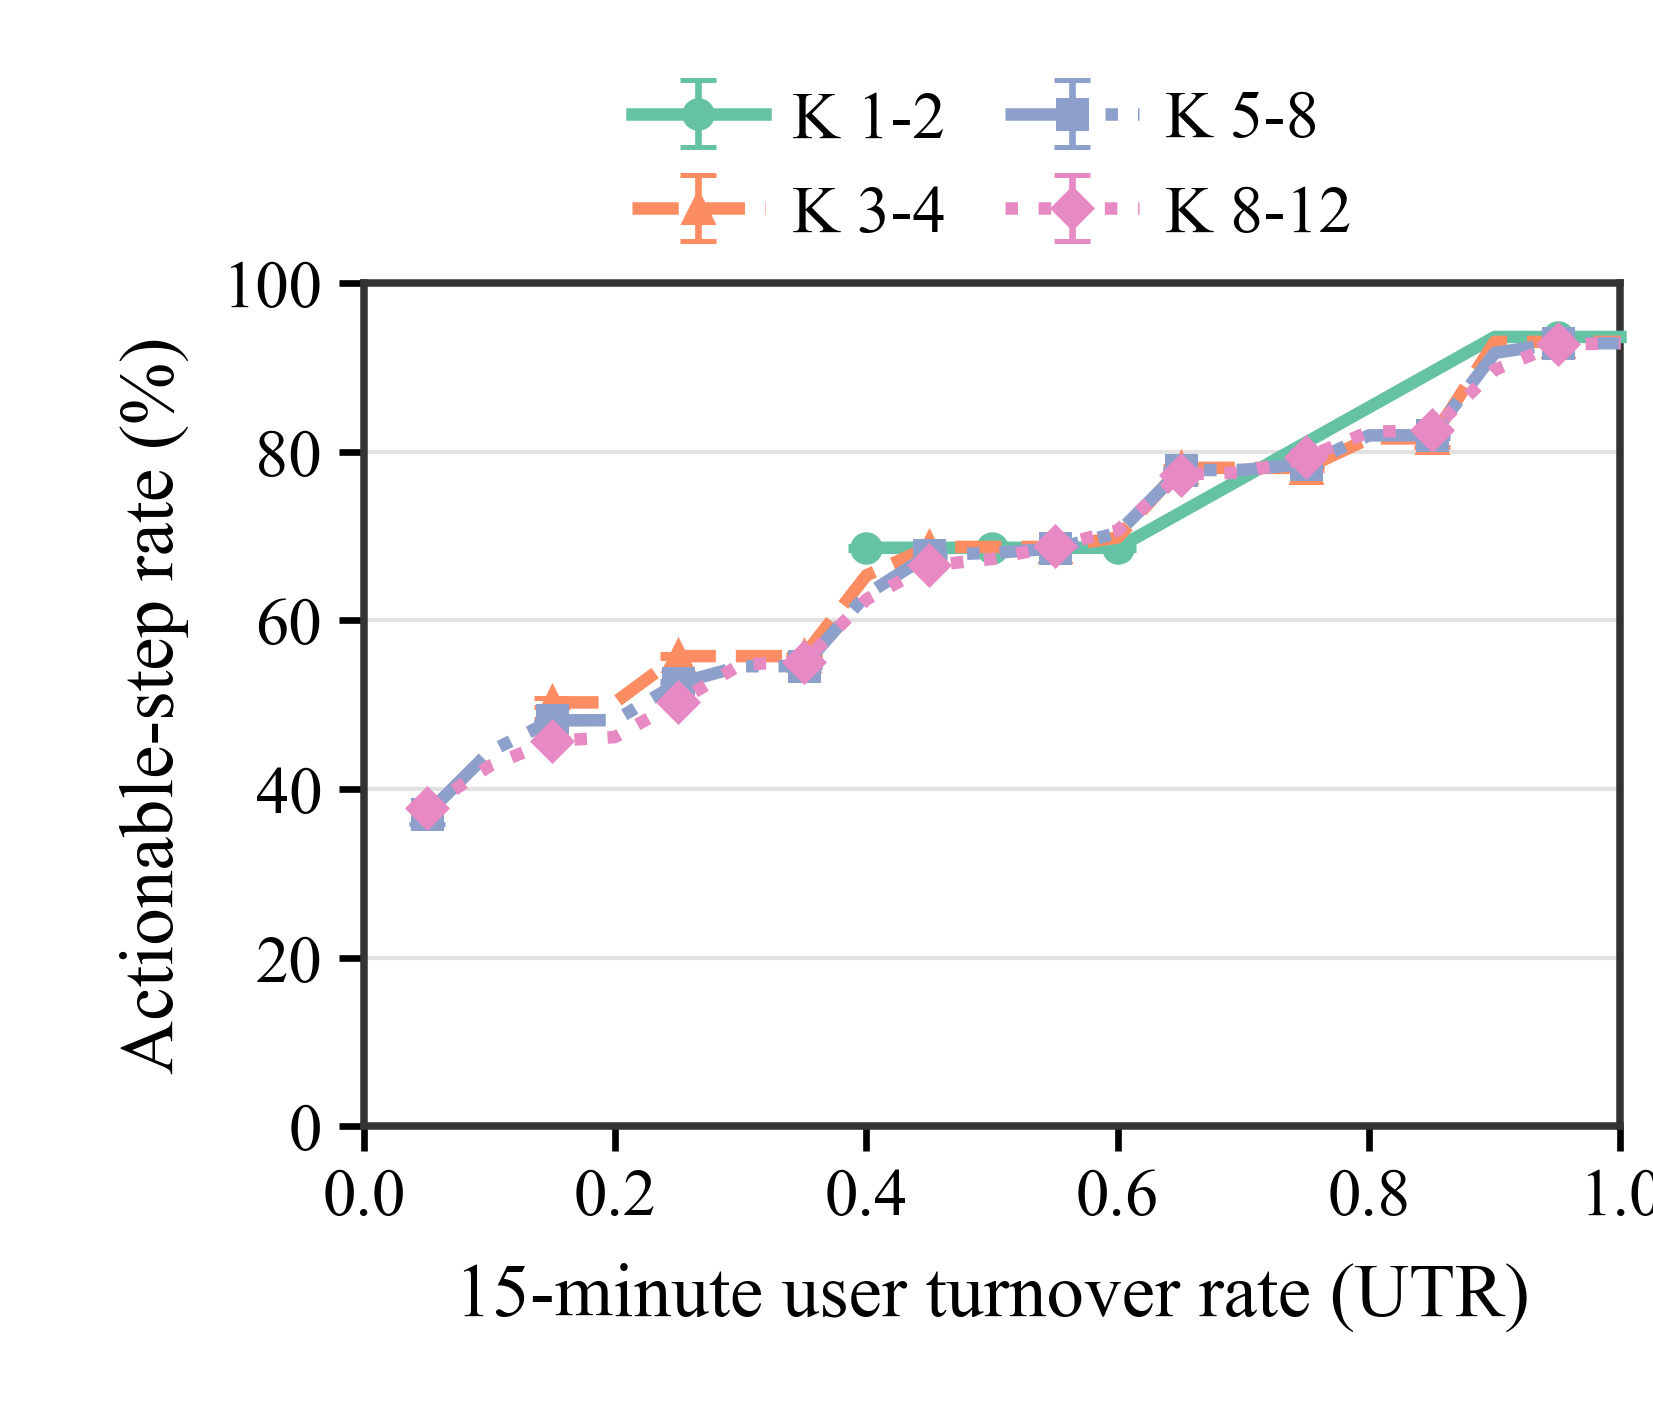
\includegraphics[width=\linewidth]{figures/fig4a_action_rate_by_turnover_compact_paper.png}
    \parbox[t]{0.96\linewidth}{\centering (a) Actionable RT-GCM update rate versus 15-minute UTR.}
  \end{minipage}\hfill
  \begin{minipage}[t]{0.49\linewidth}
    \centering
    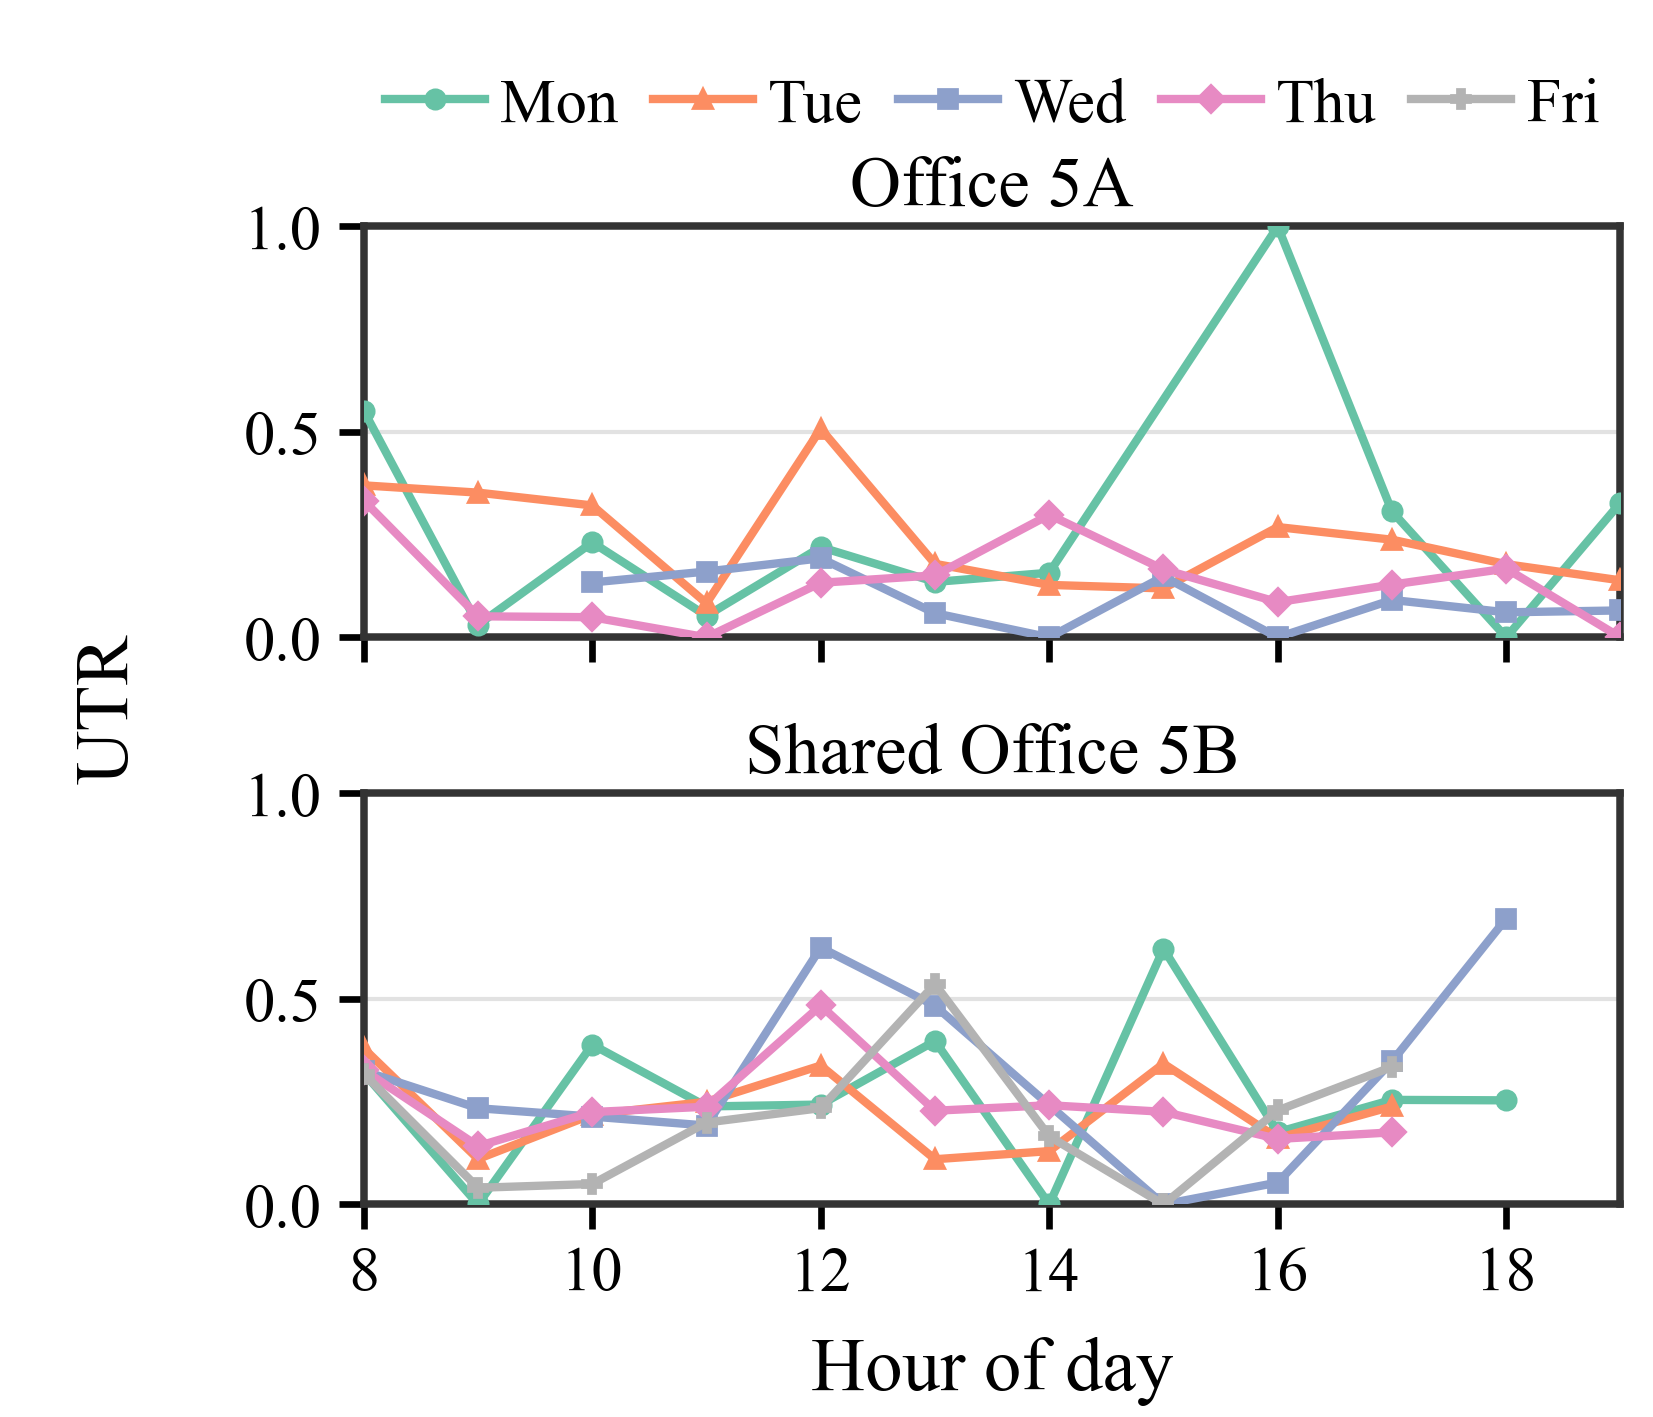
\includegraphics[width=\linewidth]{figures/fig4b_weekly_30min_utr_selected_compact_paper.png}
    \parbox[t]{0.96\linewidth}{\centering (b) Weekday 15-minute UTR profiles for selected room examples.}
  \end{minipage}
  \caption{Occupant turnover and actionable RT-GCM updates. (a) Actionable-update rate versus 15-minute UTR; an update is actionable when $|\Delta T|\geq0.5\,^{\circ}\mathrm{C}$. Lines denote bins of $K$. (b) Weekday 15-minute UTR profiles for Office 5A ($K=12$) and Shared Office 5B ($K=8$).}
  \label{fig:turnover_action}
\end{figure}
